Indexes, materialized views, and caches are crucial to query processing.
Most query processors employ one or more of these technique to speed up queries.
These technique all have a common characteristic:
they are based on the idea of maintaining additional \textit{derived state} in order to achieve more efficient read
access to data.

The use of derived state in query processing poses a number of design decisions,
which are often in tension and create trade-offs.
In this chapter, we analyze the design space of derived state based query processors.
In addition, we present a unified framework for reasoning about how these design choices interact
and how they affect the behavior of the query processor.


\section{The use of derived state in query processing}
\label{sec:read_write_path}

Secondary indexing, caching, and the use of materialized views are all instances of a common technique:
creating derived state by applying a transformation to the data stored in the database in order to accelerate particular
read access patterns to the data.

At an abstract level, derived state can be described by a \textit{write path} and a \textit{read path}
\cite{kleppmann:designing}.
\todo{illustrate with figure}
The write path is the process of creating the derived state, and keeping it up-to-date with the base data.
The read path is the process of reading from the derived state in order to perform a query processing task.
In other words, the write path is the pre-computation that takes place when a change to the base data occurs,
without knowing if the results are going to be consumed;
the read path is the computation that takes place only when it is needed for query processing.

\medskip

We can illustrate how the notion of the read and write path applies on different derived state techniques using an example.
Consider a database that stores images.
A stored image can be associated with user-defined tags, and the database provides the functionality of searching
images using queries on their tags.
Consider the query \\

\noindent
$SELECT$ $*$ $FROM$ $photoAlbum$ \\
$WHERE$ $tags.predominantColor$ $BETWEEN$ $\#0a6fb6$ $AND$ $\#52aca2$ \\

\noindent
(this query could for example be part of a service that automatically creates slideshows from the image dataset).

A secondary index on the $predominantColor$ tag can be used to facilitate this type of queries.
In this case, the write path consists of updating the secondary index when an image is inserted or deleted in the database.
The read path consists of performing an index lookup for the $predominantColor$ values in a given query,
and combining the results.

When serving the query without the use of the secondary index, the read path consists of scanning the images in $photoAlbum$,
while no tasks need to be performed when an image is inserted of deleted in the database.

Using an index moves an amount of work from the read to the write path:
less work is required for serving the query (an index lookup rather than scanning the dataset), at the expense of performing
work at each change in the dataset.

Another option for serving this query is to maintain pre-computed search results for the most common queries.
This can be implemented either as a cache, or as a materialized view.
In the case of a cache, if the query result is stored in the cache then the read path consists only of retrieving the
results from the cache;
otherwise, the read path falls back to serving the query using one of the methods described above,
and then stores the query results in the cache;
The write path may invalidate cache entries, depending on the caching policy being used.
In the case of a materialized view, the read path consists of retrieving the query results from the view,
and the write path consists of updating the view to reflect changes to the dataset.

From this example, it is clear that indexing, caching, and the use of materialized views,
can be viewed as techniques for shifting the boundaries between the read and the write path.
They allow the query processor to perform more work on the write path in order to reduce the work needed on the read path.


\section{Design decisions and trade-offs in derive state based query processing systems}

Choosing between the derived state techniques described in the previous sections,
poses a trade-off between work required on the read, and work required on the write path,
and between work on the read path and the memory and storage overhead of maintaining derived state.
These trade-offs have been studied extensively \cite{valentin:db2advisor, chaudhuri:decadeselftuning}.
Database systems provide mechanisms for managing this trade-off at runtime, by allowing the database administrator
to select indexes and materialized views to be created, and by providing mechanisms to automate this choice.

However, the use of derived state for optimizing query processing involves a number of additional design choices:
\todo{add CAP issues}
\begin{itemize}

  \item Given a change in the base data, when is the derive state updated to reflect this change?

  \item How is the derived state distributed across the system's nodes?

  \item When base data is distributed across multiple data centers, how is the derived state placed across data centers?

\todo{also mention availability of the derived state}
\end{itemize}

These design choices affect multiple aspects of the query processing system's behavior,
including query performance, overhead to write operation, relevance of query results, and operational cost.

We can reason about how these design choices interact and how they affect the query processing system's behavior
using the read and write path framework.
To do so, we first describe the tasks involved in the read and write path.
\todo{here we need a visualization}

\medskip

Given a change to the base data,
the write path consists of one or two round trip communications between the base data and the derived state
in order to propagate the changes to the base data (described in more detail in section~\ref{sec:sync_async_maintenance}),
and the computation required to apply the change to the derived state.
Similarly, given a query, the read path consists of a round trip communication between the query source (the client or a
query manager component) and a query processing computation (for example in index lookup) at the derived state.
For simplicity, we assume here simple predicate queries that do not involve more complex operations such as joins.

In a distributed database, both the base data as well as the derived state are partitioned;
Both the write and read paths may involve communication among multiple derived state and base data
partitions (section~\ref{sec:index_partitioning_design_space}).

Finally, in a geo-distributed database in which base data and derived state are distributed across multiple data centers,
both the write and read paths may involve inter- data center communication, with latencies, therefore, orders of magnitude
higher that intra- data center communication.


\subsection{Derived state maintenance schemes}
\label{sec:sync_async_maintenance}

\todo{Figure~\ref{fig:maintenance_schemes} (temporary; borrowed) redo}

Given the following update to a data item $d$:
\[
d.predominantColor = \#c78f83
\]
updating a secondary index on the $predominantColor$ attributes consists of the following steps:
\begin{enumerate}
  \item Insert $d$ to the posting list of the index entry that corresponds to $predominantColor$ $=$ $\#c78f83$.
  \item Retrieve the previous value $d.predominantColor$, for example $\#424a69$.
  \item Remove $d$ from the posting list of the index entry that corresponds to $predominantColor$ $=$ $\#424a69$.
\end{enumerate}

In practice, the derived state subscribes to the change log of the base data.
If the change log contains the information about the value of $d.attributeA$ before the change, then step (2) is not
required.

The tasks for updating a materialized view for a query on $predominantColor$ are similar.
\medskip

Given a write operation to the database,
there are different design choices for \textit{when} these steps described above are performed relative to the critical
path of the write.
We term these design choices, the derived state maintenance scheme.

In synchronous maintenance, all steps are performed in the critical path of the write operation,
usually bundled as a transaction.
This increases write latency, but ensures that derived state is always up-to-date with the base data.

An alternative approach is to perform some of the maintenance step asynchronously: deferring them for after the write
operation has been acknowledged to the client.
This reduces the overhead to write latency, but also has the implication that for each write operation
there is a time window when a data item has been updated, but the update has not been reflected in the derived state,
i.e. the derived state is stale.
Serving queries from derived state that is stale relative to the base data may result in query results with false-positives
and false-negatives.

Amazon's DynamoDB maintains its global secondary indexes asynchronously \cite{dynamodb:async}.
As a result,
applications need to ``anticipate and handle situations where a query on a secondary index returns results that are
not up to date''.


\bigskip

We can reason about derived state maintenance schemes using the framework for derived state's read and write path.
The write path can be broken down into synchronous and asynchronous tasks:
synchronous write path tasks incur overhead in write latency, while asynchronous one relax derived state's consistency
relative tho the base data.

State maintenance scheme determines the boundary between synchronous and asynchronous write path tasks.
Because asynchronous write path tasks result state derived state, and serving queries using stale derived state
introduces false-positives and false-negatives, the choice of maintenance scheme poses a trade-off between write latency
and query processing effectiveness.

\begin{figure}
  \centering

  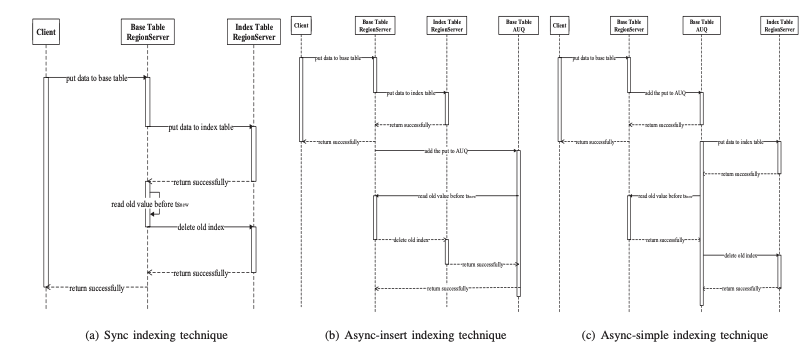
\includegraphics[width=\textwidth]{./figures/design_space/maintenance.png}

  \caption{Sequence diagram for sync (left), sync-insert (middle), async-simple (right) maintenance}

  \label{fig:maintenance_schemes}

\end{figure}

\bigskip

The following state maintenance schemes have been proposed in the literature:

\subsection{Sync-insert}
One asynchronous maintenance scheme consists of inserting new derived state entries synchronously (step 2),
and removing the old state entries asynchronously in the background (steps 2 and 3).
The literature often refers to this scheme as \textit{sync-insert}.

Sync-insert reduces the work needed to be performed at the critical path of write operations,
but it removes stale entries from the derived state in an eventually consistent fashion.
Leaving stale entries in the derived state for a time window means that query results may contain false-positives.

The sync-insert scheme is often complemented with a read-repair mechanism.
After reading from the derived state, the system removes false-positives by validating the retrieved results against
the base data.
The read-repair mechanism is a technique for shifting some work from the write to the read path.

\subsection{Async-simple}
Another asynchronous scheme, termed \textit{async-simple}, consists of acknowledging the write operation to
the client as soon as the base data is updated,
and performing all derived state maintenance steps in the asynchronously.
In practice, async-simple is implemented using an asynchronous update queue:
write operation are acknowledged as soon as they are logged in the queue;
a background process ingests the queue and performs derived state maintenance.

This scheme incurs no overhead to write operations.
However, it permits more anomalies due to applying base data changes to the derived state in an eventually consistent fashion.
More specifically, considering an update that changes $d.attributeA$ from $x$ to $y$:
\begin{itemize}
  \item If none of the state maintenance steps have been performed, $x$ will appears as the value of $d.attributeA$
  in query results.

  \item If the entry for $d.attributeA$ $==$ $x$ has been removed from the derived state, but the new value has not been
  inserted, $d$ will appear to have been removed from the dataset

  \item If the entry for $d.attributeA$ $==$ $y$ has been added to the derived state, but the old value has not been
  removed, $d.attributeA$ will appear to have two values
\end{itemize}

% Diff-Index \cite{tan:diffindex} has proposed an asynchronous index maintenance scheme that provides sessions guarantees.
% The technique used to achieve this is to track additional state in the client library:
% this state is used to guarantee that any index look-up contains updates to the base data that were made in the same
% session.
% This guarantees the read-your-writes property.

\subsection{Derived state partitioning}
\label{sec:index_partitioning_design_space}

\todo{Figures~\ref{fig:prob1_6_2} and~\ref{fig:prob1_6_1} (temporary; borrowed) redo}

Scaling derived state both in terms size and and read access requires partitioning it across multiple system nodes.
In chapter chapter~\ref{ch:background}, we presented the two main index partitioning schemes.

Briefly, the main index partitioning schemes are:
\begin{itemize}

  \item In \textbf{partitioning by document}, index entries are co-located in the same node as the corresponding
  data items.

  \item In \textbf{partitioning by term}, a global index is partitioned with the same partitioning scheme as the base data,
  using the indexed value as partitioning key.

\end{itemize}

The same partitioning schemes can be applied to a materialized view.
In the rest of this section we refer to secondary indexes.
The same results apply to Materialized views.

\medskip

In the partitioning-by-document approach, an index lookup requires broadcasting a read request to every index partition
and then gathering the returned results.
On the other hand, when reading from a term-partitioned index only the index partitions with index entries that are
relevant to the query need to be contacted.
In term-partitioned index, however, an additional round of messages is required for retrieving the base data items,
as they may be located on different nodes that the corresponding index entries (assuming the index does not contain a
replica of the base data)
This is not the case for the document-partitioned index, since data items are by-design co-located with the corresponding
index entries.

An advantage of the document-partitioned index is that updating the index upon a write to the database does not require
communication between nodes.
On the other hand, updating a term-partitioned index may involve significant communication overhead, as an update to data
item may involve updating index entries located on different nodes.

\bigskip

These observations can be grouped under the framework of derived state's read and write path.
Partitioning-by-document guarantees local-only communication on the write path, but requires a large volume of
communication on the read path (a scatter/gather operation involving all partitions);
Partitioning-by-term involves communication across nodes on the write path (a change to data item may need to be sent to
an index partition on another node),
but requires less communication on the read path in the general case
(index partitions known do not include relevant index entries are not contacted).

\begin{figure}
    \centering
    \begin{minipage}{.5\textwidth}
        \centering
        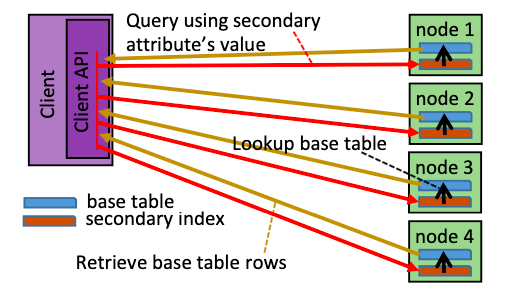
\includegraphics[scale=0.3]{figures/design_space/communication_pattern_document_partitioned.png}
        \caption{}
        \label{fig:prob1_6_2}
    \end{minipage}%
    \begin{minipage}{0.5\textwidth}
        \centering
        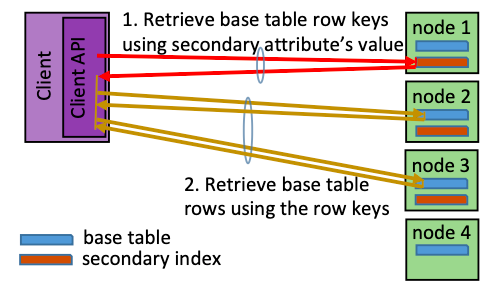
\includegraphics[scale=0.3]{figures/design_space/communication_pattern_term_partitioned.png}
        \caption{}
        \label{fig:prob1_6_1}
    \end{minipage}
\end{figure}

Guided by this analysis we can reason about the performance characteristics of the two approaches.

Partitioning-by-document is more suitable at a small scale (small number of nodes),
while partitioning-by-term becomes more suitable as the number of nodes increases,
and has been shown to provide better scalability \cite{kejriwal:slik}.

In addition to the system's architecture scale,
which approach is more suitable depends on a number of different workload characteristics.
In \cite{dsilva:tworings}, D`silva et al. perform an extensive experimental comparison of the two approaches,
implemented in HBase, and show how various workload characteristic affect the index partitioning scheme's performance.

Key factors that affect index lookup performance are:
\begin{itemize}

  \item The distribution of the values of the indexed attribute:
  As the number of data items per index value increase, partitioning-by-document performs better.
  This is because of the additional round trip required to retrieve the base data items:
  as the number of data items per index value increases, a term-partitioned index is likely to have to contact
  more and more remote nodes, while in a document-partitioned index data items are always co-located on the same node as
  the index entries.

  \item Concurrency:
  As the number of concurrent index lookups increases, partitioning-by-term performs better.
  This can be attributed to the overhead of the scatter/gather operation used by the document-partitioned index:
  As the volume of concurrent index lookups increases,
  the overhead of broadcasting to every node becomes more significant.

  \item The selectivity of queries:
  The document-partitioned index outperforms the term-partitioned index as the range size in range queries increases.
  This is in accordance with the observation that partitioning-by-document is beneficial when there are
  more records to be returned.

\end{itemize}

In addition, this work assumes synchronous index maintenance, and evaluates the impact of the two approach to write
operations.
The document-partitioned index generally outperforms the term-partitioned for writes,
incurring less overhead to write latency and providing better scalability.

From the above analysis it is evident that neither of the two approaches is suitable for all needs.
The choice of which approach to use should be guided by factors including the scale of the system,
the properties of the dataset (distribution of indexed values over the data items),
and the characteristics of the workload (query/write ratio, concurrency, query selectivity)
\todo{note also that this work does not consider the significant latencies involved in geo-distribution. This exaggerates the effects}

More specifically:
\begin{itemize}

  \item Partitioning-by-document is more suitable for:
  (1) smaller scale systems with a small number of nodes and light index lookup concurrency,
  (2) workloads with less selective queries that return large result sets,
  (3) skewed data distribution where a large number of data items have the same indexed value,
  or (4) write-intensive workloads.

  \item Term-partitioned indexes are more suitable for:
  (1) larger scale systems with a greater number of nodes,
  (2) query-intensive workloads with a large query load,
  (3) workloads consisting of more selective queries with smaller result sets,
  or (4) data with normal distribution of the indexed value.

\end{itemize}

Clearly, the decision of which index partitioning approach to be used needs be taken in a case-by-case basis.
Database systems should to support both index partitioning schemes, and expose the partitioning scheme selection as a
configuration parameter at the time of creating an index.
We are not aware of any database system that provides this functionality.
In existing systems, this design decision is made at design time, and every index uses the same partitioning scheme.
\cite{kejriwal:slik, tan:diffindex, riakv:secondaryindexes, cassandra:secondaryindexing}
In Section~\ref{sec:cs_index_partitioning} we demonstrate how a distributed database can provide both index partitioning
schemes.


\subsection{Derived state topology patterns}
\label{sec:topology_patterns}
\todo{not a good title: should include the term ``placement''}

% \todo{discuss existing approaches for placement of query processing operators across servers for minimizing cross-server communication}

In our analysis, we have made the implicit assumption so far that base data and derived state are placed in the
same date center, and that clients are located in the same geographic region,
and that communication latency among them is not significant.
However, in modern cloud-scale services this is often not the case.
Users are often spread across multiple geographic locations.
As a result, database systems distribute data across geographically distributed data centers,
in order to reduce latencies and improve fault-tolerance.

Long-distance inter- data center network links exhibit latencies in the order of tens to hundreds of milliseconds.
This is an order of magnitude higher than intra- data center latencies as well as latencies perceived by users served
from a data center close to their location \cite{kleppmann:localfirst}.

In this setting, design choices about the placement of derived state,
and about the communication patterns between with base data and derived state and between derived state and clients
determine whether the read and write path computations require intra- or inter- data center communication.
We refer to these design choices \textit{topology patterns}.

Design choices related to inter- data center communication exacerbate the trade-offs presented in the previous sections,
but also pose additional trade-offs related to derived state replication.

In this section, we discuss a number of scenarios that involve geo-distribution, and the associated derived state
topology patterns.
Throughout the following sections we consider as an example the design choices involved in maintaining a secondary index,
however the analysis can also be applied to materialized views.

\subsubsection{Geo-replication}
Cloud-scale database systems rely on geo-distribution to minimize user-perceived latency and improve fault-tolerance.
This architecture poses a design choice which stems from an impossibility property, known as the CAP theorem
\cite{brewer:cap}.
in the face of network partitions between data centers, geo-replicated databases must choose between strongly consistent
(CP) and high-available (AP) designs.
In a strongly-consistent design, replicas are kept synchronized at all times.
This provides the abstraction of single replica system which simplifies application logic, but exposes users to high
latencies due to the need for inter- data center communication between replicas in the critical path of each write
operation.
In addition, strongly-consistent designs are susceptible to downtimes due to network partitions.
In a highly-available design, replicas synchronize in the background, out of the critical path of write operations.
This ensures low latency and availability under network partitions, as each replica serves write operations locally.
Nevertheless, this allows replicas to accept concurrent conflicting updates and temporary diverge.

\medskip

We first consider a strongly-consistent design.
One approach is to maintain a replica of the materialized view on each data center.
With this approach, both the read and write path involve only intra- data center communication.
Queries can be served from the materialized view at the closest date center.
Moreover, since the entire dataset is present on each data center,
keeping materialized view replicas up-to-date with the base data requires only intra- data center communication.
The downside of this approach is the storage overhead associated with maintaining multiple replicas of the materialized
view.

An alternative approach is to have materialized view replicas only on some data centers.
This reduces the storage overhead, but means that a query sent to a data center without a materialized view
either needs to be forwarded to another data center, or processed without the use of a materialized view,
both of which result in slower query processing.
This can be suitable for case in which some data centers are queried more often than others.
Moreover, this approach can be supplemented with the use of caches in data centers without materialized
views.

\medskip

TODO: here we need a paragraph about AP.
Mainly, discuss conflicts and derived data.

\subsubsection{Geo-partitioning}
A different geo-distribution strategy is geo-partitioning.
In geo-partitioning, data is partitioned across data centers, and partitions are placed on data centers according to
their access patterns.
As a result, latency read and write access to data that belong to a local partition is low.
CockroachDB allows developers to partition data across data centers with row-level granularity
\cite{cockroachdb:geopartitioning}.

One approach for maintaining a secondary index over geo-partitioned data is to use the partitioning-by-document scheme:
each data center maintains a secondary index covering only the data items in local partitions.
This approach has the same implication as document-based partitioning:
the write path only requires intra- data center communication, since the index is co-located with the base data;
the read path needs to contact every index partition and gather results, which requires inter- data center
communication.

A different approach is to maintain a global secondary index on each data center.
In that case, the index lookups (read path) can always be served on the local data center.
However, each change to the base data need to be propagated to all data centers (write path).
The downside of this approach is that it significantly increases the storage cost.

\subsubsection{Multi-cloud and Query federation}
More recently, the concept of multi-cloud data storage has emerged.
Organizations spread their data across private data centers and public cloud services in order to reduce costs and
ensure fault-tolerance.
Moreover, they distribute data across multiple cloud providers in order to avoid dependence on a single
cloud provider, take advantage of diverse storage and computing services, and improve reliability.

The advent of data distributed across multiple independent storage systems has created the need for unified access and
federated search across platforms.
The problem of federated query processing can be viewed as a generalization of the geo-partitioning case:
the dataset at each platform can be seen as a partition of the logical global dataset.
For simplicity, we assume that a multi-cloud platform consists of multiple, independent instances of a common database
system.
Under there assumptions, the same design decisions and trade-offs as in the case of geo-partitioning apply to query
federation across multiple clouds.
The same observations can be generalized to heterogeneous systems composed of different database system.
However, federated query processing includes additional challenges linked to the heterogeneous data models of these
systems.

\bigskip

From the examples above it becomes clear that topology patterns play a major role in the performance of geo-distributed
query processing based on derived state

\section{Conclusion (placeholder title)}

\todo{we need a vizualization \\ multi-dimensional table? decision tree? something else?}

\begin{itemize}
  \item The use of derived state to speed-up query processing moves query processing work from the read path to the write
  path, while also incurring memory and storage overhead.
  Moreover, different derived state schemes (indexes, materialized views, caching) entail different amount of work
  on the read and write path.

  \item The choice of derived state maintenance scheme controls the impact of work on the write path:
  Synchronous maintenance keeps the derived state up-to-date with the base data,
  but incurs overhead to the latency of write operations.
  On the other hand, asynchronous maintenance schemes move some of the work on the write path in the background.
  This reduces the overhead to write operations, but also means that derived state is not always up-to-date with the base
  data.
  Because serving queries from derived state that is stale relative to the base data may introduce false-positive and
  false-negatives,
  design decisions on derived state maintenance pose a trade-off between the overhead to write operations
  and the relevance of query results.

  \item The derived state partitioning scheme determines the communication pattern between base data and derived state
  on the write path, and between derived state and client on the read path.
  More specifically, partitioning-by-document ensures that no cross-node communication is needed on the write path,
  but requires a scatter/gather operation across all state partitions on the read path.
  Partitioning-by-term requires cross-node communication on the write path but reduces the number of state partitions
  that need to participate on the read path.
  Therefore, the choice of partitioning scheme poses a trade-off in the type (intra-node or cross-node) and volume
  of communication on the read versus the write path.

  \item When base data and client are distributed across different geographic locations,
  the choice of topology pattern affects the communication latency (intra versus inter data center communication).
  This creates a number of trade-offs, that result from the basic trade-off of requiring intra data center communication
  on the read versus the write path.
  These trade-offs include:
  \begin{itemize}
    \item Low latency on the read path versus increased latency on the write path in the case of synchronous maintenance,
    or decreased freshness in the case of asynchronous maintenance.
    \item Low latency on the read path versus increased resource utilization for maintaining derived state replicas,
    and increased volume of write path communication.
    \item Low data transfer cost on the read path versus on the write path.
  \end{itemize}

\end{itemize}